% AThesis v2.2

% این قالب بر اساس فرمت پایان‌نامه‌ها و رساله‌های تحصیلات تکمیلی دانشگاه صنعتی اصفهان تهیه شده است.

% ارسال نظرات جهت بهبود قالب:
% a101.fakhari@gmail.com

% توصیه می‌شود که از توزیع تک‌لایو (TexLive) استفاده شود:
% http://tug.org/texlive/acquire-iso.html

% از نصب بودن فونت B ZAR و B Zar Bold بر روی سیستم خود اطمینان حاصل کنید. اگر به مشکل پیدا نکردن فونت برخوردید، از وجود این فونت ها در پوشه Windows/Fonts از طریق CMD مطمین شوید.
% کمپایلر ادیتور را روی XeLaTeX قرار دهید.

% موفق باشید.
% امین فخاری
% ‌دی‌ماه 1394
% -----------------------------------------------------------------------------------

% نکات:

% برای آن‌که پردازش فایل و مشاهده خروجی در هنگام نوشتن پایان‌نامه آسان‌تر و سریع‌تر انجام شود، انجام موارد زیر توصیه می گردد:
% الف) فصل‌ها و بخش‌هایی که در حال نوشتن آن‌ها نیستید را غیر فعال کنید. به‌عنوان مثال، در این قالب، این دستورات را می‌توان در صورت عدم نیاز با اضافه کردن % به طور موقت غیرفعال کرد:
% \MakeTitlePage
% \MakeFarsiSignaturePage
% \clearpage
\thispagestyle{empty}
\newgeometry{left=3cm,right=4cm,top=7cm}

{\BZarScaleOne
{\fontsize{20pt}{0}\selectfont
\noindent
% عنوان تشکر و قدردانی---------------------------------------------------------
تشکر و قدردانی
% ؛---------------------------------------------------------
}}
\vspace{0.5cm}

{\BZarScaleOne
{\fontsize{12pt}{0.9cm}\selectfont % Zar 13
\noindent
% متن تشکر و قدردانی---------------------------------------------------------
خدایا تو را شاکرم به خاطر امروزم که به من عطا فرمودی...






% ؛---------------------------------------------------------
}}

\restoregeometry
% \MakeCopyRightPage
% \clearpage
\thispagestyle{empty}
\newgeometry{left=3cm,right=4cm,top=7cm}

{\BZarScaleOne
{\fontsize{28pt}{0}\selectfont
\noindent
% تقدیم اثر---------------------------------------------------------
تقـدیم به
\\[1cm]
\hspace*{1cm}
همسرم به مهربانی فرشته
% ؛---------------------------------------------------------
}}
		
\restoregeometry
% \MakeTableOfContents
% \MakeListOfFigures
% \MakeListOfTables
% \MakeFarsiAbstract
% \input{Chapters/Chapter#}
% \MakeAppendices
% \section{جزئیات معادله‌ها}
نوشته نمونه نوشته نمونه نوشته نمونه نوشته نمونه نوشته نمونه نوشته نمونه نوشته نمونه نوشته نمونه نوشته نمونه نوشته نمونه نوشته نمونه نوشته نمونه نوشته نمونه نوشته نمونه نوشته نمونه نوشته نمونه نوشته نمونه نوشته نمونه نوشته نمونه نوشته نمونه نوشته نمونه نوشته نمونه. نوشته نمونه نوشته نمونه نوشته نمونه نوشته نمونه نوشته نمونه نوشته نمونه نوشته نمونه نوشته نمونه نوشته نمونه نوشته نمونه نوشته نمونه نوشته نمونه نوشته نمونه نوشته نمونه نوشته نمونه نوشته نمونه نوشته نمونه نوشته نمونه نوشته نمونه نوشته نمونه نوشته نمونه نوشته نمونه. نوشته نمونه نوشته نمونه نوشته نمونه نوشته نمونه نوشته نمونه نوشته نمونه نوشته نمونه نوشته نمونه نوشته نمونه نوشته نمونه نوشته نمونه نوشته نمونه نوشته نمونه نوشته نمونه نوشته نمونه نوشته نمونه نوشته نمونه نوشته نمونه نوشته نمونه نوشته نمونه نوشته نمونه نوشته نمونه. نوشته نمونه نوشته نمونه نوشته نمونه نوشته نمونه نوشته نمونه نوشته نمونه نوشته نمونه نوشته نمونه نوشته نمونه نوشته نمونه نوشته نمونه نوشته نمونه نوشته نمونه نوشته نمونه نوشته نمونه نوشته نمونه نوشته نمونه نوشته نمونه نوشته نمونه نوشته نمونه نوشته نمونه نوشته نمونه. نوشته نمونه نوشته نمونه نوشته نمونه نوشته نمونه نوشته نمونه نوشته نمونه نوشته نمونه نوشته نمونه نوشته نمونه نوشته نمونه نوشته نمونه نوشته نمونه نوشته نمونه نوشته نمونه نوشته نمونه نوشته نمونه نوشته نمونه نوشته نمونه نوشته نمونه نوشته نمونه نوشته نمونه نوشته نمونه. نوشته نمونه نوشته نمونه نوشته نمونه نوشته نمونه نوشته نمونه نوشته نمونه نوشته نمونه نوشته نمونه نوشته نمونه نوشته نمونه نوشته نمونه نوشته نمونه نوشته نمونه نوشته نمونه نوشته نمونه نوشته نمونه نوشته نمونه نوشته نمونه نوشته نمونه نوشته نمونه نوشته نمونه نوشته نمونه. نوشته نمونه نوشته نمونه نوشته نمونه نوشته نمونه نوشته نمونه نوشته نمونه نوشته نمونه نوشته نمونه. نمونه‌ای از یک رابطه به‌صورت
\begin{equation}
p\left( r \right) = {C_k}\frac{N}{{\pi {a^2}}}{\left[{1 - {{\left( {\frac{r}{a}} \right)}^k}} \right]^{\frac{1}{k}}}
\label{Eq:Pressure1}
\end{equation}
است.

\newpage
\section{اثبات روابط ریاضی}
نوشته نمونه نوشته نمونه نوشته نمونه نوشته نمونه نوشته نمونه نوشته نمونه نوشته نمونه نوشته نمونه نوشته نمونه نوشته نمونه نوشته نمونه نوشته نمونه نوشته نمونه نوشته نمونه نوشته نمونه نوشته نمونه نوشته نمونه نوشته نمونه نوشته نمونه نوشته نمونه نوشته نمونه نوشته نمونه. نوشته نمونه نوشته نمونه نوشته نمونه نوشته نمونه نوشته نمونه نوشته نمونه نوشته نمونه نوشته نمونه نوشته نمونه نوشته نمونه نوشته نمونه نوشته نمونه نوشته نمونه نوشته نمونه نوشته نمونه نوشته نمونه نوشته نمونه نوشته نمونه نوشته نمونه نوشته نمونه نوشته نمونه نوشته نمونه. نوشته نمونه نوشته نمونه نوشته نمونه نوشته نمونه نوشته نمونه نوشته نمونه نوشته نمونه نوشته نمونه نوشته نمونه نوشته نمونه نوشته نمونه نوشته نمونه نوشته نمونه نوشته نمونه نوشته نمونه نوشته نمونه نوشته نمونه نوشته نمونه نوشته نمونه نوشته نمونه نوشته نمونه نوشته نمونه. (شکل~%
\ref{Fig:World1})
نوشته نمونه نوشته نمونه نوشته نمونه نوشته نمونه نوشته نمونه نوشته نمونه نوشته نمونه نوشته نمونه نوشته نمونه نوشته نمونه نوشته نمونه نوشته نمونه نوشته نمونه نوشته نمونه نوشته نمونه نوشته نمونه نوشته نمونه نوشته نمونه نوشته نمونه نوشته نمونه نوشته نمونه نوشته نمونه. نوشته نمونه نوشته نمونه نوشته نمونه نوشته نمونه نوشته نمونه نوشته نمونه نوشته نمونه نوشته نمونه نوشته نمونه نوشته نمونه نوشته نمونه نوشته نمونه نوشته نمونه نوشته نمونه نوشته نمونه نوشته نمونه نوشته نمونه نوشته نمونه نوشته نمونه نوشته نمونه نوشته نمونه نوشته نمونه. نوشته نمونه نوشته نمونه نوشته نمونه نوشته نمونه نوشته نمونه نوشته نمونه نوشته نمونه نوشته نمونه نوشته نمونه نوشته نمونه نوشته نمونه نوشته نمونه نوشته نمونه نوشته نمونه نوشته نمونه نوشته نمونه نوشته نمونه نوشته نمونه نوشته نمونه نوشته نمونه نوشته نمونه نوشته نمونه.
\begin{figure}[!htb]
\centering
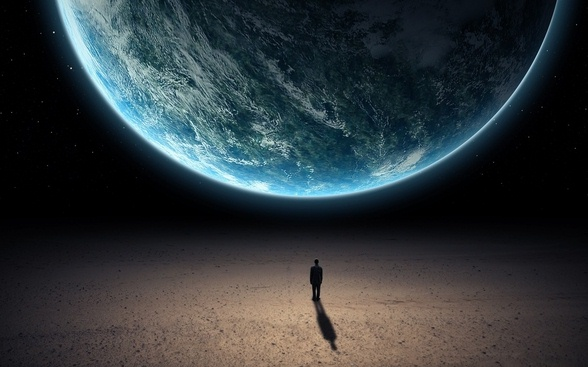
\includegraphics[scale=0.4]{Figures/World.jpg}
\caption{تصویر مفهومی}
\label{Fig:World1}
\end{figure}

نوشته نمونه نوشته نمونه نوشته نمونه نوشته نمونه نوشته نمونه نوشته نمونه نوشته نمونه نوشته نمونه نوشته نمونه نوشته نمونه نوشته نمونه نوشته نمونه نوشته نمونه نوشته نمونه نوشته نمونه نوشته نمونه نوشته نمونه نوشته نمونه نوشته نمونه نوشته نمونه نوشته نمونه نوشته نمونه.
% \MakeEnglishAbstract
% \MakeEnglishSignaturePage
% ب) از گزینه draft برای فراخوانی کلاس استفاده کنید. یعنی
% \documentclass[a4paper,fleqn,10pt,oneside,draft]{book}
% این گزینه حالت چرکنویس را ایفا می‌کند و بر روی بسته‌های مختلف اثرهای متفاوتی دارد. به‌عنوان مثال: به جای شکل، تنها چهارچوب آن نمایش داده شود، لینک‌های hyperref غیر فعال گردد، فایل‌های خارجی را در بسته listings اضافه نمی‌کند و ... و همه این موارد سبب کاهش زمان اجرا و حجم فایل می‌شود.

% در صورتی که میخواهید به سطر بعد بروید اما نمیخواهید بین دو کلمه‌ای که نوشتید فاصله بیفتد کافی است در انتهای خط اول  (بدون فاصله) کاراکتر % را اضافه کنید. با این عمل، لاتک خط فاصله ایجاد شده در اثر تغییر سطر را به عنوان توضیح اضافه یا کامنت در نظر میگیرد و در خروجی اعمال نمی‌کند.

% توصیه می‌شود از شکل‌های برداری با فرمت PDF استفاده شود. این کار علاوه بر افزایش کیفیت رسال/پایان‌نامه/گزارش، باعث کاهش حجم شکل‌ها (و در نتیجه  کاهش حجم فایل نهایی) و همچنین کاهش زمان پردازش می‌شود.

% در این قالب سعی شده است که از تمامی بخش‌های موجود در پایان‌نامه‌ها نمونه‌ای آورده شود.

\documentclass[a4paper,fleqn,10pt,oneside]{book}
%-----------------------------
% بسته‌های دلخواه را در این قسمت اضافه نمایید:

%-----------------------------
\usepackage{Settings/AThesisStyle}
%-----------------------------
% دستورهای مورد نیاز را در این قسمت اضافه نمایید:

%-----------------------------

\begin{document}

\pagestyle{plain}
\pagenumbering{adadi}
\setcounter{page}{2}

% ░░░░░░░▒▒▒▒▒▒▓▓▓▓ In the Name of Allah ▓▓▓▓▒▒▒▒▒▒░░░░░░░
\clearpage
\thispagestyle{empty}
\begin{figure}[t]
\centering

\includegraphics[scale=1.3]{Settings/Allah.pdf}
\end{figure}

% ░░░░░░░▒▒▒▒▒▒▓▓▓▓ Title Page ▓▓▓▓▒▒▒▒▒▒░░░░░░░
\DepartmentFa{دانشکده مهندسی مکانیک}
\ThesisTypeFa{رساله} % Or \ThesisTypeFa{پایان‌نامه} Or \ThesisTypeFa{پیشنهادیه پایان‌نامه}
\DegreeFa{دکتری} % Or \DegreeFa{کارشناسی ارشد}
\FieldFa{مهندسی مکانیک}
\YourFullnameFa{امین فخاری}
\FirstSupervisorFa{دکتر مهدی کشمیری}
\SecondSupervisorFa{دکتر راهنمای دوم} % Optional (Remove It If You Don't Have)
\YearFa{1394}
\TitleFa{
تحلیل و کنترل لغزش در جابجایی اجسام در تماس با سطوح هموار
\\[0.4cm]
توسط انگشتان نرم
}
% اگر عنوان رساله طولانی بود، در دو خط به صورت نشان داده شده تقسیم شود.

\MakeTitlePage

% ░░░░░░░▒▒▒▒▒▒▓▓▓▓ Signature - Farsi ▓▓▓▓▒▒▒▒▒▒░░░░░░░
\Prefix{آقای} %\Prefix{خانم}
\DateFa{1394/10/6}
\FirstAdvisorFa{دکتر مشاور اول}
\SecondAdvisorFa{دکتر مشاور دوم} % Optional (Remove It If You Don't Have)
\FirstExaminerFa{دکتر داور اول}
\SecondExaminerFa{دکتر داور دوم} % Optional (Remove It If You Don't Have)
\ThirdExaminerFa{دکتر داور سوم} % Optional (Remove It If You Don't Have)
\FourthExaminerFa{دکتر داور چهارم} % Optional (Remove It If You Don't Have)
\FifthExaminerFa{دکتر داور پنجم} % Optional (Remove It If You Don't Have)
\DeanOfDepartmentFa{دکتر تحصیلات تکمیلی دانشکده}

\MakeFarsiSignaturePage

% ░░░░░░░▒▒▒▒▒▒▓▓▓▓ Acknowledgments ▓▓▓▓▒▒▒▒▒▒░░░░░░░
\clearpage
\thispagestyle{empty}
\newgeometry{left=3cm,right=4cm,top=7cm}

{\BZarScaleOne
{\fontsize{20pt}{0}\selectfont
\noindent
% عنوان تشکر و قدردانی---------------------------------------------------------
تشکر و قدردانی
% ؛---------------------------------------------------------
}}
\vspace{0.5cm}

{\BZarScaleOne
{\fontsize{12pt}{0.9cm}\selectfont % Zar 13
\noindent
% متن تشکر و قدردانی---------------------------------------------------------
خدایا تو را شاکرم به خاطر امروزم که به من عطا فرمودی...






% ؛---------------------------------------------------------
}}

\restoregeometry

% ░░░░░░░▒▒▒▒▒▒▓▓▓▓ CopyRight ▓▓▓▓▒▒▒▒▒▒░░░░░░░
\MakeCopyRightPage

% ░░░░░░░▒▒▒▒▒▒▓▓▓▓ Dedication ▓▓▓▓▒▒▒▒▒▒░░░░░░░
\clearpage
\thispagestyle{empty}
\newgeometry{left=3cm,right=4cm,top=7cm}

{\BZarScaleOne
{\fontsize{28pt}{0}\selectfont
\noindent
% تقدیم اثر---------------------------------------------------------
تقـدیم به
\\[1cm]
\hspace*{1cm}
همسرم به مهربانی فرشته
% ؛---------------------------------------------------------
}}
		
\restoregeometry

% ░░░░░░░▒▒▒▒▒▒▓▓▓▓ Table of Contents/Figures/Tables ▓▓▓▓▒▒▒▒▒▒░░░░░░░
\MakeTableOfContents
\MakeListOfFigures
\MakeListOfTables

% ----------------------------------------------------------------------------
\clearpage
\pagestyle{myheadings}
\pagenumbering{arabic}
\setcounter{page}{1}

% ░░░░░░░▒▒▒▒▒▒▓▓▓▓ Abstract - Farsi ▓▓▓▓▒▒▒▒▒▒░░░░░░░
\AbstractFa{
در این قسمت چکیده‌ی فارسی پایان‌نامه نوشته می‌شود. در این قسمت چکیده‌ی فارسی پایان‌نامه نوشته می‌شود. در این قسمت چکیده‌ی فارسی پایان‌نامه نوشته می‌شود. در این قسمت چکیده‌ی فارسی پایان‌نامه نوشته می‌شود. در این قسمت چکیده‌ی فارسی پایان‌نامه نوشته می‌شود. در این قسمت چکیده‌ی فارسی پایان‌نامه نوشته می‌شود. در این قسمت چکیده‌ی فارسی پایان‌نامه نوشته می‌شود. در این قسمت چکیده‌ی فارسی پایان‌نامه نوشته می‌شود. در این قسمت چکیده‌ی فارسی پایان‌نامه نوشته می‌شود. در این قسمت چکیده‌ی فارسی پایان‌نامه نوشته می‌شود. در این قسمت چکیده‌ی فارسی پایان‌نامه نوشته می‌شود. در این قسمت چکیده‌ی فارسی پایان‌نامه نوشته می‌شود. در این قسمت چکیده‌ی فارسی پایان‌نامه نوشته می‌شود. در این قسمت چکیده‌ی فارسی پایان‌نامه نوشته می‌شود. در این قسمت چکیده‌ی فارسی پایان‌نامه نوشته می‌شود. در این قسمت چکیده‌ی فارسی پایان‌نامه نوشته می‌شود. در این قسمت چکیده‌ی فارسی پایان‌نامه نوشته می‌شود. در این قسمت چکیده‌ی فارسی پایان‌نامه نوشته می‌شود. در این قسمت چکیده‌ی فارسی پایان‌نامه نوشته می‌شود. در این قسمت چکیده‌ی فارسی پایان‌نامه نوشته می‌شود. در این قسمت چکیده‌ی فارسی پایان‌نامه نوشته می‌شود. در این قسمت چکیده‌ی فارسی پایان‌نامه نوشته می‌شود. در این قسمت چکیده‌ی فارسی پایان‌نامه نوشته می‌شود. در این قسمت چکیده‌ی فارسی پایان‌نامه نوشته می‌شود. در این قسمت چکیده‌ی فارسی پایان‌نامه نوشته می‌شود. در این قسمت چکیده‌ی فارسی پایان‌نامه نوشته می‌شود. در این قسمت چکیده‌ی فارسی پایان‌نامه نوشته می‌شود. در این قسمت چکیده‌ی فارسی پایان‌نامه نوشته می‌شود. در این قسمت چکیده‌ی فارسی پایان‌نامه نوشته می‌شود. در این قسمت چکیده‌ی فارسی پایان‌نامه نوشته می‌شود.‎‎
}

\KeywordsFa{
1-کلمه‌ی کليدی اوّل،  2-کلمه‌ی کليدی دوم ، 3-کلمه‌ی کليدی سوم،  4-کلمه‌ی کليدی چهارم، 5-کلمه‌ی کليدی پنجم
}
\MakeFarsiAbstract

% ░░░░░░░▒▒▒▒▒▒▓▓▓▓ Chapters ▓▓▓▓▒▒▒▒▒▒░░░░░░░
\clearpage
\baselineskip=0.9cm

\chapter{مقدمه}
\section{پیش‌گفتار}
در این قالب سعی شده است که از تمامی بخش‌های موجود در پایان‌نامه‌ها نمونه‌ای آورده شود. در این قالب سعی شده است که از تمامی بخش‌های موجود در پایان‌نامه‌ها نمونه‌ای آورده شود. در این قالب سعی شده است که از تمامی بخش‌های موجود در پایان‌نامه‌ها نمونه‌ای آورده شود. در این قالب سعی شده است که از تمامی بخش‌های موجود در پایان‌نامه‌ها نمونه‌ای آورده شود. در این قالب سعی شده است که از تمامی بخش‌های موجود در پایان‌نامه‌ها نمونه‌ای آورده شود. در این قالب سعی شده است که از تمامی بخش‌های موجود در پایان‌نامه‌ها نمونه‌ای آورده شود. در این قالب سعی شده است که از تمامی بخش‌های موجود در پایان‌نامه‌ها نمونه‌ای آورده شود. در این قالب سعی شده است که از تمامی بخش‌های موجود در پایان‌نامه‌ها نمونه‌ای آورده شود. در این قالب سعی شده است که از تمامی بخش‌های موجود در پایان‌نامه‌ها نمونه‌ای آورده شود. در این قالب سعی شده است که از تمامی بخش‌های موجود در پایان‌نامه‌ها نمونه‌ای آورده شود. در این قالب سعی شده است که از تمامی بخش‌های موجود در پایان‌نامه‌ها نمونه‌ای آورده شود. در این قالب سعی شده است که از تمامی بخش‌های موجود در پایان‌نامه‌ها نمونه‌ای آورده شود. در این قالب سعی شده است که از تمامی بخش‌های موجود در پایان‌نامه‌ها نمونه‌ای آورده شود. در این قالب سعی شده است که از تمامی بخش‌های موجود در پایان‌نامه‌ها نمونه‌ای آورده شود.
\section{بخش اول}
نمونه‌ای از یک عبارت انگلیسی در متن به‌صورت
\lr{English Sentence}
است. نمونه‌ای از یک عبارت ریاضی در متن نیز به‌صورت
$x^2 + y^2$
است. ارجاع به مراجع انگلیسی
\cite{Fakhari2015a,Lewis2003}.
ارجاع به مراجع فارسی
\cite{Fakhari2015b,HadianThesis2008}.
این نمونه‌ای از یک زیرنویس انگلیسی%
\LTRfootnote{English Footnote}
است. این نمونه‌ای از یک زیرنویس فارسی%
\RTLfootnote{زیرنویس فارسی}
است. در شکل
\ref{Fig:SampleFigure1}،
نمونه‌ای از یک شکل آورده شده است. 

\begin{figure}[!htb]
\centering
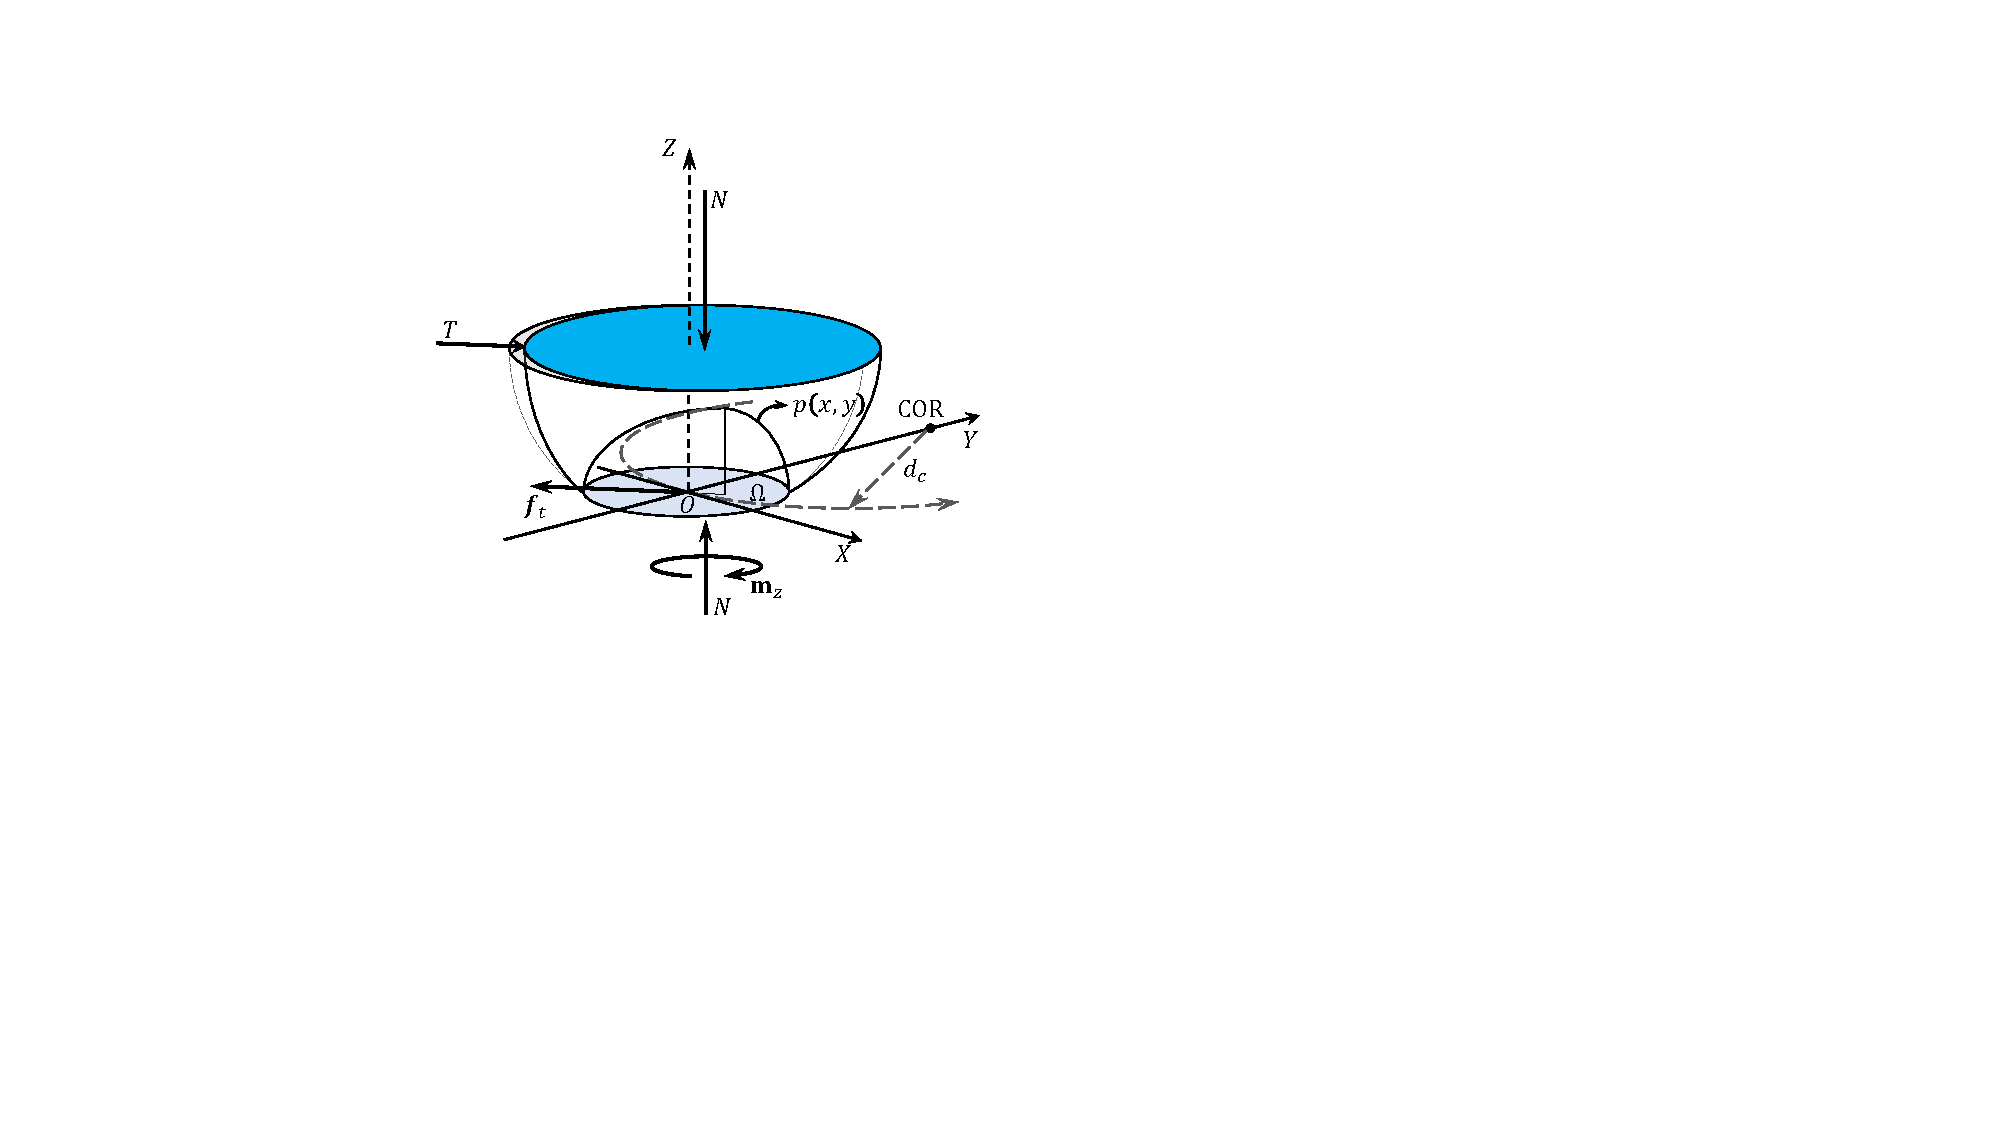
\includegraphics[scale=1]{Figures/SampleFigure.pdf}
\caption{شکل نمونه}
\label{Fig:SampleFigure1}
\end{figure}

نمونه‌ای از قرار دادن دو شکل در کنار یکدیگر در شکل
\ref{Fig:SampleFigure2}
آورده شده است.

\begin{figure}[!htb]
\centering
\subfloat[زیرنویس شکل اول]{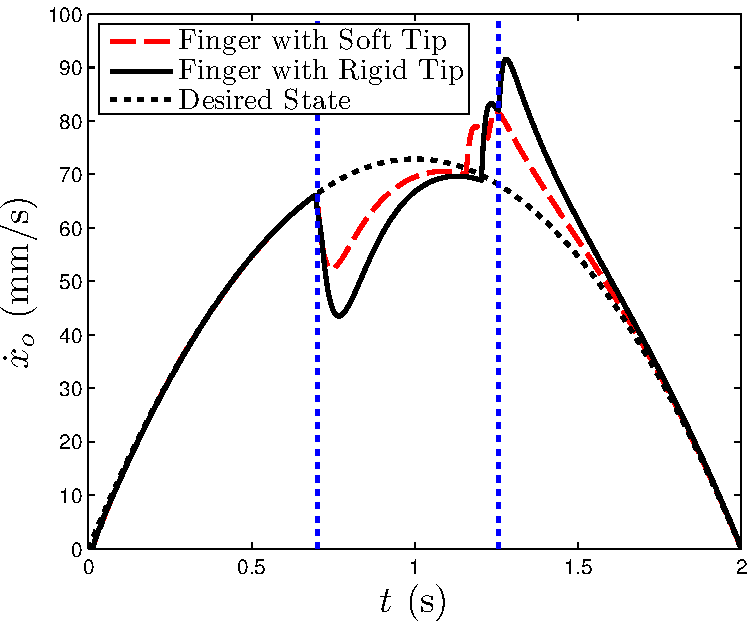
\includegraphics[scale=0.56]{Figures/FigureA.pdf}}
\quad
\subfloat[زیرنویس شکل دوم]{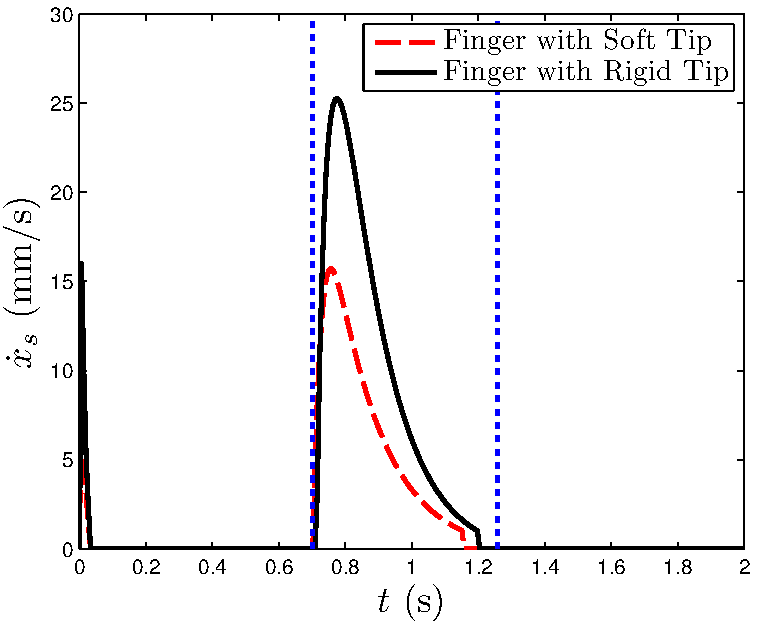
\includegraphics[scale=0.56]{Figures/FigureB.pdf}}
\caption{
قرار دادن دو شکل در کنار یکدیگر، الف) شکل نمونه اول،
ب) شکل نمونه دوم
}
\label{Fig:SampleFigure2}
\end{figure}





آیتم‌های مختلف به‌صورت زیر آورده می‌شود:
\begin{itemize}[label=-]
\item
مورد اول
\item
مورد دوم
\item
مورد سوم
\end{itemize}

نمونه‌ای از آیتم‌های شماره‌دار نیز در ادامه آورده شده است. به طور کلی معماری برداشت انرژی به دو دسته‌ی کلی تقسیم می‌شود:
\begin{enumerate}[label=\arabic*)]
\item
برداشت-استفاده:

در این حالت سیستم بلافاصله انرژی برداشت‌شده را مصرف می‌کند. واضح است اگر انرژی کافی در محیط وجود نداشته باشد دستگاه از کار می‌افتد. این نوع سیستم‌ها بیشتر در فشار دادن کلید‌ها، پدال‌ها و دستگاه‌های ردیابی برای انسان‌ها استفاده می‌شود. به طور مثال در پاشنه‌ی کفش دونده‌ای مواد پیزوالکتریک کار گذاشته می‌شود و با فشار پا بر روی کفش و فشرده شدن پیزوالکتریک داخل کفش، انرژی الکتریکی برای ارسال سیگنال 
\lr{RF}
و در نتیجه ردیابی دونده تامین می‌شود. 
\item
برداشت-ذخیره-استفاده:

در این روش سیستم برای ذخیره‌ی انرژی برداشت‌شده به باتری مجهز شده است. این روش برای زمانی‌که انرژی زیادی در محیط وجود داشته باشد و برای منابعی مانند انرژی خورشیدی  کاربرد دارد. روش‌های زیادی برای تبدیل انرژی خورشیدی به انرژی الکتریکی از جمله سلول‌های خورشیدی وجود دارد. در این حالت چگونگی ذخیره‌ی انرژی و بهینه‌سازی مصرف انرژی مطرح می‌شود.
\end{enumerate}




\subsection{زیربخش اول}
نوشته نمونه نوشته نمونه نوشته نمونه نوشته نمونه نوشته نمونه نوشته نمونه نوشته نمونه نوشته نمونه نوشته نمونه نوشته نمونه نوشته نمونه نوشته نمونه نوشته نمونه نوشته نمونه نوشته نمونه نوشته نمونه نوشته نمونه نوشته نمونه نوشته نمونه نوشته نمونه نوشته نمونه نوشته نمونه. در جدول
\ref{Tbl:SampleTable1}،
نمونه‌ای از یک جدول واردشده در لاتک و در جدول
\ref{Tbl:SampleTable2}،
نمونه‌ای از یک جدول نوشته‌شده در لاتک آورده شده است.

\begin{table}[!htb]
\caption{پارامترهای شبیه‌سازی}
\centering
\begin{tabular}{c}
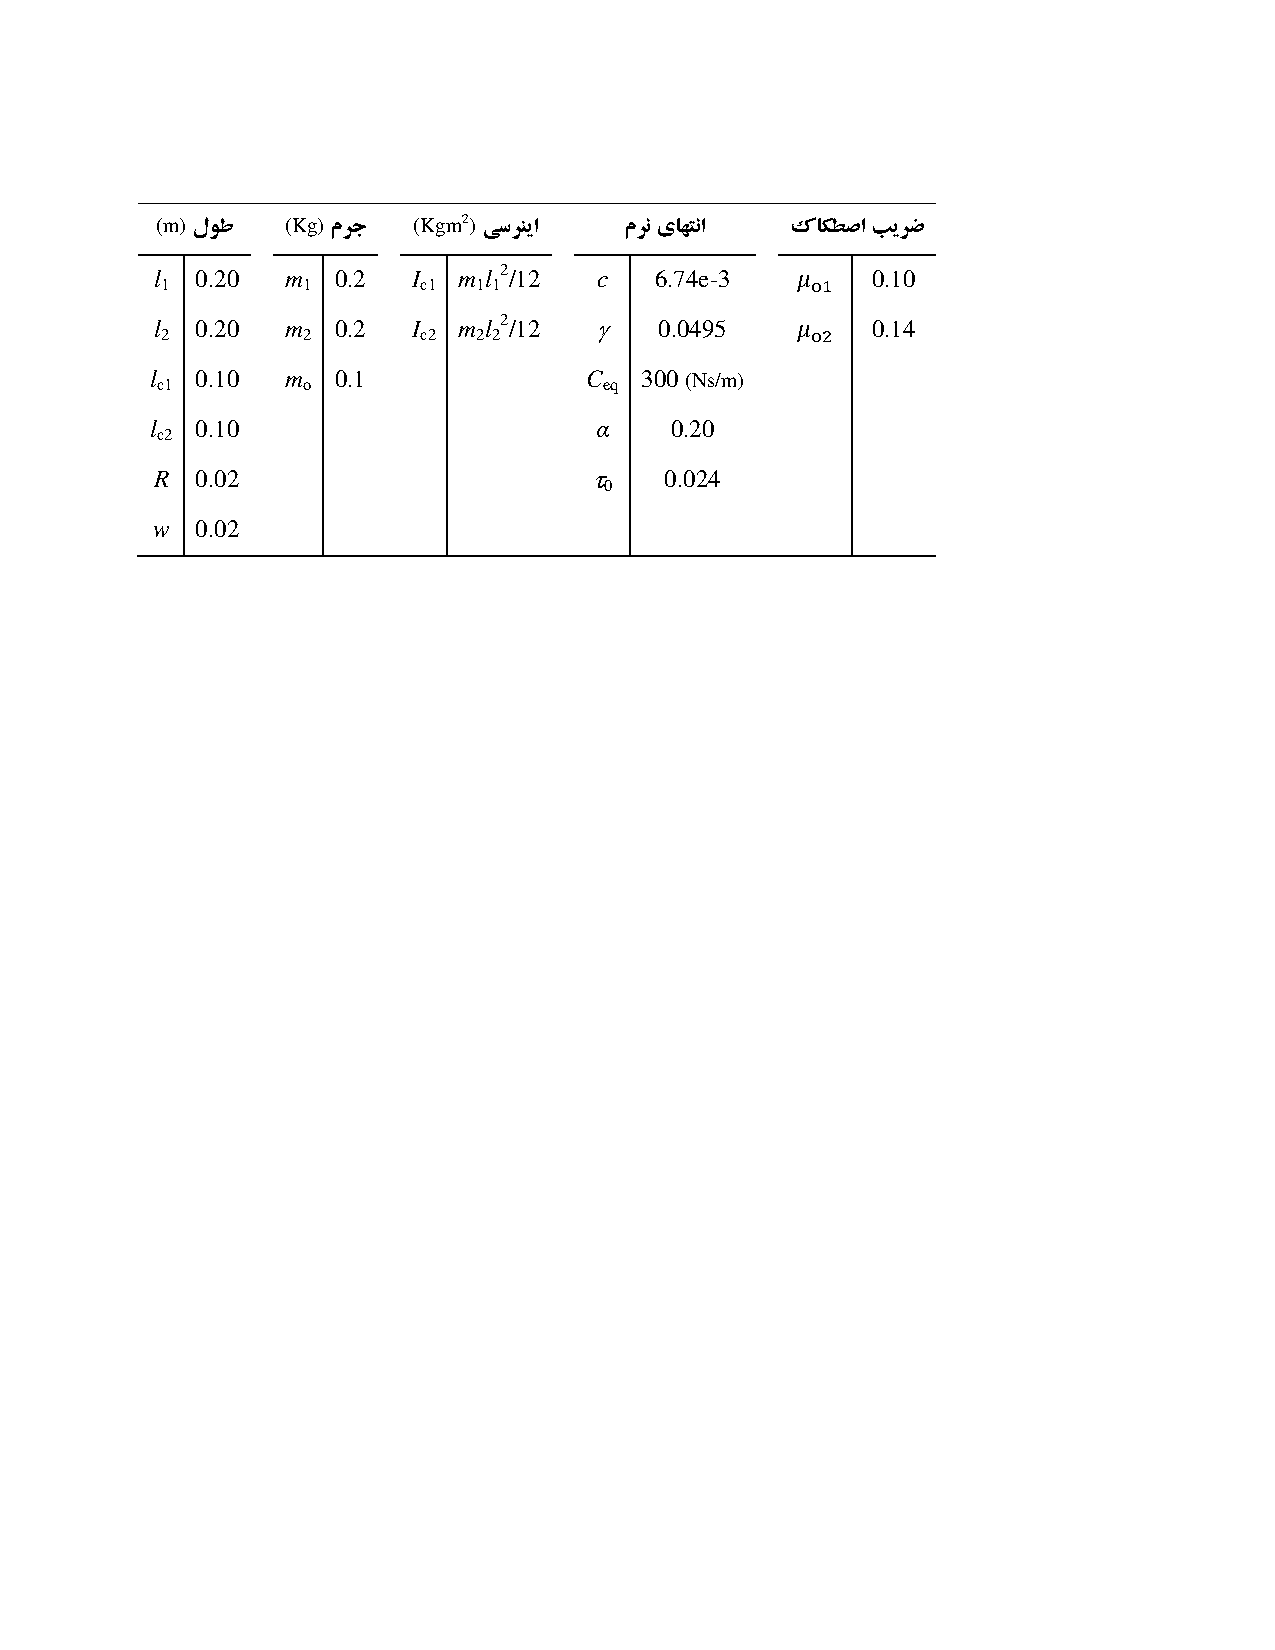
\includegraphics[scale=0.9]{Figures/SampleTable1.pdf} 
\end{tabular}
\vspace{-\baselineskip}
\label{Tbl:SampleTable1}
\end{table}

\begin{table}[!htb]
\caption{مقايسه‌ی روش‌هاي برداشت انرژي مبتني بر لرزش‌هاي مکانيکی}
\centering
\begin{tabular}{@{}|p{.15\textwidth}|p{.25\textwidth}|p{.25\textwidth}|p{.25\textwidth}|@{}}
\hline
روش
& 
چگالی انرژی
& 
ابعاد
& 
عیب اصلی
\\ \hline \hline
پیزوالکتریک
& 
$\mathrm{mJ/cm^3}$ 35/4
& 
بزرگ
& 
ولتاژ خروجی کم
\\ \hline
الکترومغناطیس
& 
$\mathrm{mJ/cm^3}$ 24/8
& 
بزرگ
& 
ولتاژ خروجی بسیار کم
\\ \hline
الکترواستاتیک
& 
$\mathrm{mJ/cm^3}$ 4
& 
فشرده در تراشه‌ها
& 
نیاز به منبع شارژ اولیه
\\ \hline
\end{tabular}
\label{Tbl:SampleTable2}
\vspace{-\baselineskip}
\end{table}

نمونه‌ای از یک رابطه به‌صورت
\begin{equation}
p\left( r \right) = {C_k}\frac{N}{{\pi {a^2}}}{\left[{1 - {{\left( {\frac{r}{a}} \right)}^k}} \right]^{\frac{1}{k}}},
\label{Eq:Pressure}
\end{equation}
است. در رابطه
\ref{Eq:Pressure}،
$N$
نیروی عمودی است. نمونه‌ای از استفاده از روابط متوالی به‌صورت
\begin{equation}
\sum \limits_{i = 1}^{k + 1} {E_s}\left( i \right) - T \sum \limits_{i = 1}^k {P_s}\left( i \right) \le B_s^{max},\quad k = 1, \ldots ,N - 1,
\label{Eq:batterysource}
\end{equation}\vspace{-\baselineskip}
\begin{equation}
\sum \limits_{i = 1}^{k + 1} {E_r}\left( i \right) - T \sum \limits_{i = 1}^k {P_r}\left( i \right) \le B_r^{max},\quad k = 1, \ldots ,N - 1,
\label{Eq:batteryrellay}
\end{equation}
است. نمونه‌ای از یک قضیه و تبصره نیز در ادامه آورده شده است.
\begin{theorem}
اگر ظرفیت باتری‌ها به اندازه کافی بزرگ باشد، جواب بهینه‌ی 
$P_s^*(i)$
و
$P_r^*(i)$
وجود دارد به نحوی که تابع هدف را بیشینه می‌کند و در رابطه‌ی زیر صدق می‌کند:
\begin{equation}
C\left( {{{\left| {{h_{sr}}\left( i \right)} \right|}^2}{P_s}^*\left( i \right)} \right) \ge C\left( {{{\left| {{h_{sd}}\left( i \right)} \right|}^2}{P_s}^*\left( i \right)} \right) + C\left( {{{\left| {{h_{rd}}\left( {i + 1} \right)} \right|}^2}P_r^*\left( {i} \right)} \right).
\label{Eq:theorem1}
\end{equation}

\begin{proof}
بار دیگر فرم تابع هدف را در نظر می‌گیریم. لازم به ذکر است اینجا تابع هدف یک تابع دومتغیره است.
\begin{equation}
{R({\mathbf{P}_s},{\mathbf{P}_r}) = {\frac{1}{2}\sum\limits_{i = 1}^N {\min } \left\{ {C\left( {{{\left| {{h_{sr}}\left( i \right)} \right|}^2}{P_s}\left( i \right)} \right),} C\left( {{{\left| {{h_{sd}}\left( i \right)} \right|}^2}{P_s}\left( i \right)} \right) \right\} }}.
\end{equation}
حال بلوک
$i$ام
را در نظر می‌گیریم. اگر رابطه‌ی
\ref{Eq:theorem1}
برای
$i$
برقرار نباشد، به عبارت دیگر اگر داشته باشیم،
\begin{equation}
C\left( {{{\left| {{h_{sr}}\left( i \right)} \right|}^2}{P_s}^*\left( i \right)} \right) < C\left( {{{\left| {{h_{sd}}\left( i \right)} \right|}^2}{P_s}^*\left( i \right)} \right) + C\left( {{{\left| {{h_{rd}}\left( {i + 1} \right)} \right|}^2}P_r^*\left( {i + 1} \right)} \right),
\label{Eq:theorem1(2)}
\end{equation}
بنابراین
\begin{equation}
C\left( {{{\left| {{h_{sr}}\left( i \right)} \right|}^2}{P_s}^*\left( i \right)} \right)+ C\left( {{{\left| {{h_{sd}}\left( i \right)} \right|}^2}{P_s}^*\left( i \right)} \right) =C\left( {{{\left| {{h_{sr}}\left( i \right)} \right|}^2}{P_s}^*\left( i \right)} \right).
\end{equation}
پس در تابع هدف مسئله، مقدار بهینه‌ی مسئله برابر عبارت سمت چپ رابطه‌ی
\ref{Eq:theorem1(2)}
شده است و آرگومان دوم و  هم‌چنین مقدار
$P_r^*(i)$
هیچ نقشی در مقدار بهینه ندارد. بنابراین می‌توانیم 
$P_r^*(i)$
را آنقدر کاهش دهیم تا در رابطه‌ی
\ref{Eq:theorem1(2)}
تساوی برقرار شود بدون آنکه مقدار بهینه‌ی مسئله تغییر کند.
\end{proof}
\label{theorem1}
\end{theorem}

\begin{remark}
از قضیه‌ی
\ref{theorem1}
نتیجه می‌گیریم که جواب بهینه‌ی مسئله‌ی
\lr{P}
در حالت کلی یکتا نیست. به طور مثال وقتی مقدار انرژی برداشت‌شده در رله خیلی بیشتر از این انرژی در منبع باشد مسئله می‌تواند جواب‌های زیادی داشته باشد. بنابراین همواره می‌توان برای صرفه‌جویی در مصرف انرژی، بدون کاهش مقدار نرخ گذردهی سیستم، کمترین مقدار توان را برای رله انتخاب کرد. بنابراین با توجه به رابطه
\begin{equation}
C\left( {{{\left| {{h_{sr}}\left( i \right)} \right|}^2}{P_s}^*\left( i \right)} \right) 
\ge C\left( {{{\left| {{h_{sd}}\left( i \right)} \right|}^2}{P_s}^*\left( i \right)} \right) + C\left( {{{\left| {{h_{rd}}\left( {i} \right)} \right|}^2}P_r^*\left( {i} \right)} \right),
\label{Eq:remark1}
\end{equation}
و با  استفاده از رابطه
\ref{Eq:remark1}
خواهیم داشت،
\begin{equation}
{R_r}(i) = \min \left\{ {C\left( {{{\left| {{h_{rd}}(i)} \right|}^2}{P_r}(i)} \right),C\left( {{{\left| {{h_{sr}}(i)} \right|}^2}{P_s}(i)} \right)} \right\}.
\end{equation}

بنابراین می‌توان با انتخاب کمترین توان و نرخ برای رله از مصرف بی‌رویه‌ی انرژی جلوگیری کرد. فرض بزرگ بودن ظرفیت باتری‌ به این دلیل است که اگر ظرفیت باتری محدود باشد برای کاهش
$P_r^*(i)$
با محدودیت مواجه هستیم. چون در صورت کاهش بی از حد توان رله ممکن است از ناحیه‌ی شدنی مسئله خارج شویم. به هر حال برای هر دو حالت ظرفیت نامحدود و محدود باتری جواب مسئله یکتا نیست و همواره می‌توان با کاهش توان رله مصرف انرژی را کاهش داد.
\end{remark}





\chapter{مطالب اصلی}
\section{پیش‌گفتار}
در این قالب سعی شده است که از تمامی بخش‌های موجود در پایان‌نامه‌ها نمونه‌ای آورده شود. در این قالب سعی شده است که از تمامی بخش‌های موجود در پایان‌نامه‌ها نمونه‌ای آورده شود. در این قالب سعی شده است که از تمامی بخش‌های موجود در پایان‌نامه‌ها نمونه‌ای آورده شود. در این قالب سعی شده است که از تمامی بخش‌های موجود در پایان‌نامه‌ها نمونه‌ای آورده شود. در این قالب سعی شده است که از تمامی بخش‌های موجود در پایان‌نامه‌ها نمونه‌ای آورده شود. در این قالب سعی شده است که از تمامی بخش‌های موجود در پایان‌نامه‌ها نمونه‌ای آورده شود. در این قالب سعی شده است که از تمامی بخش‌های موجود در پایان‌نامه‌ها نمونه‌ای آورده شود. در این قالب سعی شده است که از تمامی بخش‌های موجود در پایان‌نامه‌ها نمونه‌ای آورده شود. در این قالب سعی شده است که از تمامی بخش‌های موجود در پایان‌نامه‌ها نمونه‌ای آورده شود. در این قالب سعی شده است که از تمامی بخش‌های موجود در پایان‌نامه‌ها نمونه‌ای آورده شود. در این قالب سعی شده است که از تمامی بخش‌های موجود در پایان‌نامه‌ها نمونه‌ای آورده شود. در این قالب سعی شده است که از تمامی بخش‌های موجود در پایان‌نامه‌ها نمونه‌ای آورده شود. در این قالب سعی شده است که از تمامی بخش‌های موجود در پایان‌نامه‌ها نمونه‌ای آورده شود. در این قالب سعی شده است که از تمامی بخش‌های موجود در پایان‌نامه‌ها نمونه‌ای آورده شود.
\section{بخش اول}
نمونه‌ای از یک عبارت انگلیسی در متن به‌صورت
\lr{English Sentence}
است. نمونه‌ای از یک عبارت ریاضی در متن نیز به‌صورت
$x^2 + y^2$
است. ارجاع به مراجع انگلیسی
\cite{Fakhari2015a,Lewis2003}.
ارجاع به مراجع فارسی
\cite{Fakhari2015b,HadianThesis2008}.
این نمونه‌ای از یک زیرنویس انگلیسی%
\LTRfootnote{English Footnote}
است. این نمونه‌ای از یک زیرنویس فارسی%
\RTLfootnote{زیرنویس فارسی}
است. در شکل
\ref{Fig:SampleFigure1_2}،
نمونه‌ای از یک شکل آورده شده است. 

\begin{figure}[!htb]
\centering
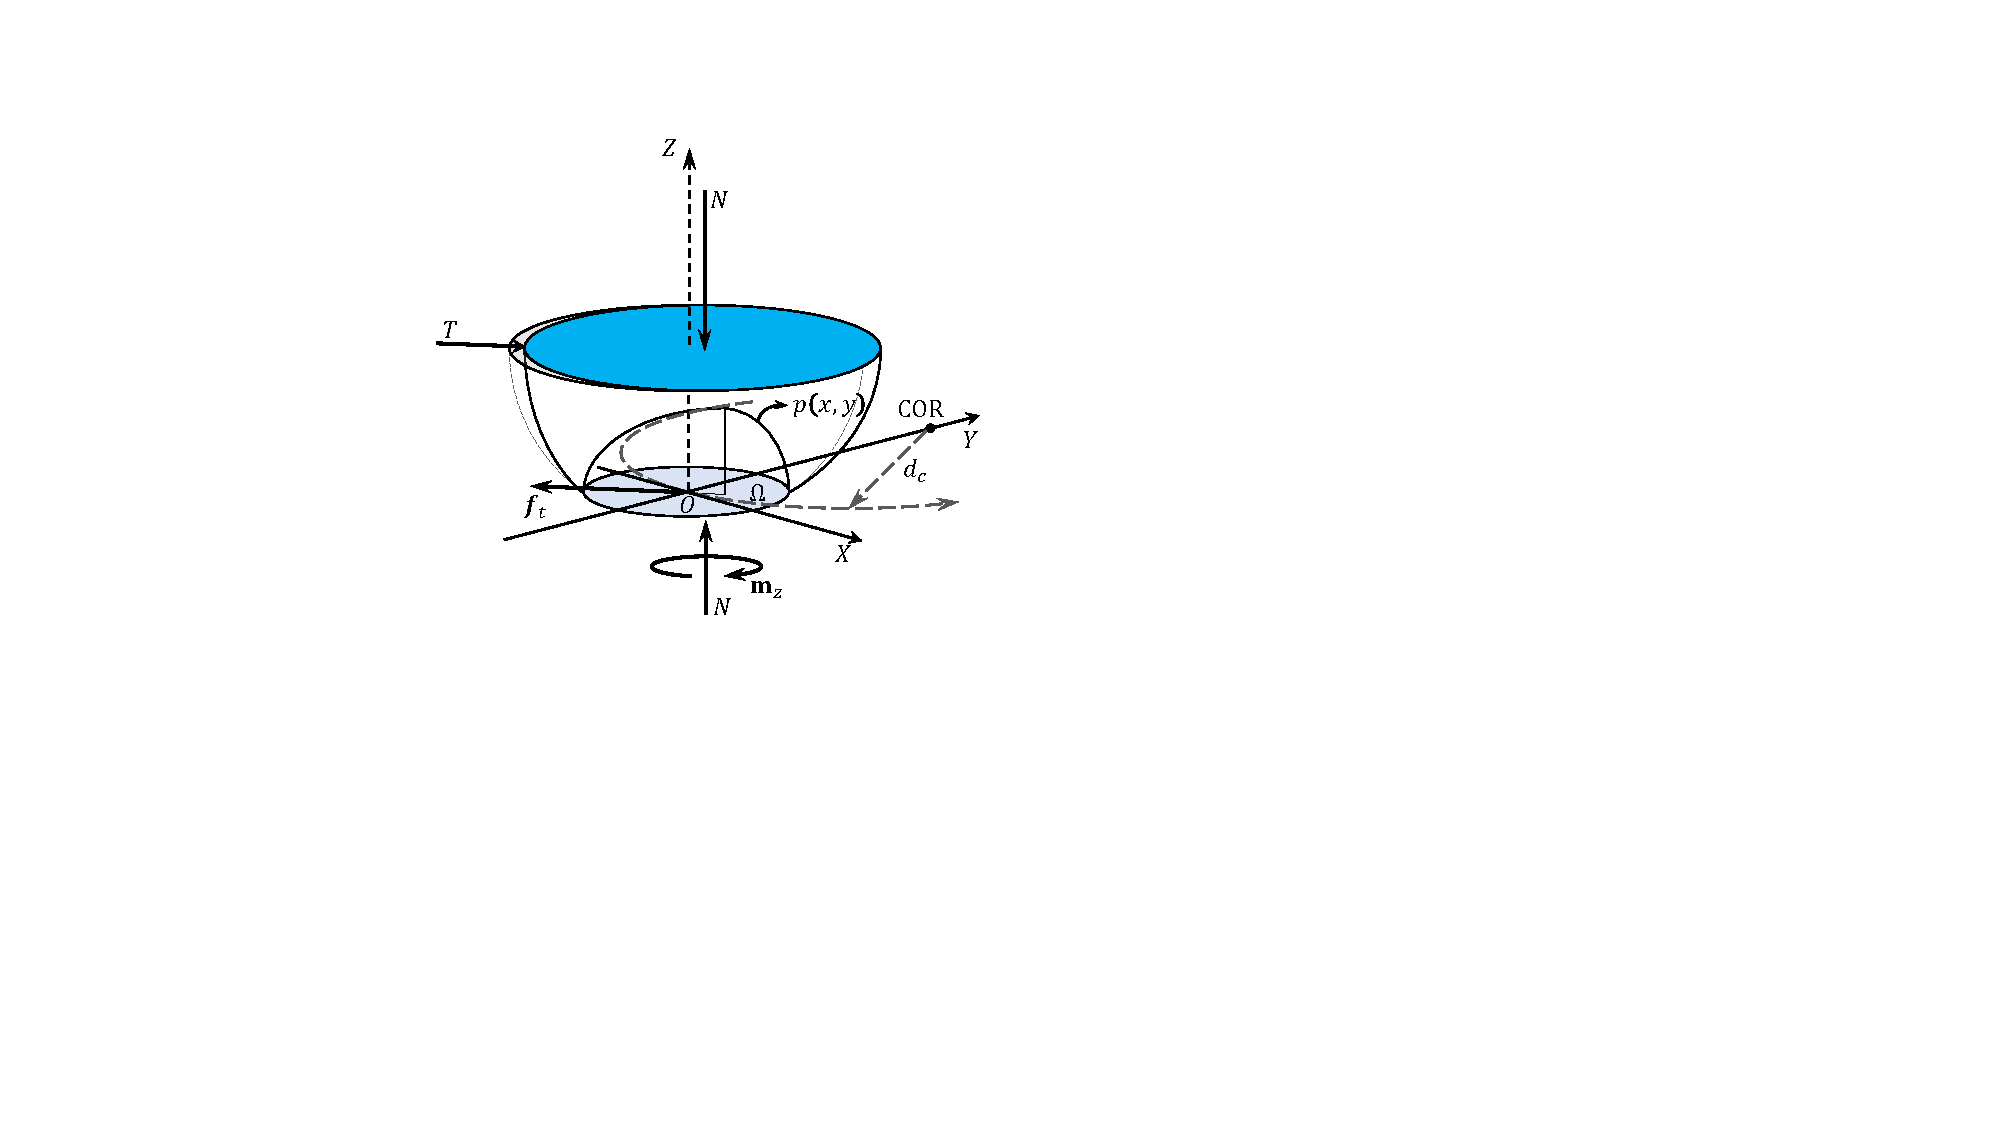
\includegraphics[scale=1]{Figures/SampleFigure.pdf}
\caption{شکل نمونه}
\label{Fig:SampleFigure1_2}
\end{figure}

نمونه‌ای از قرار دادن دو شکل در کنار یکدیگر در شکل
\ref{Fig:SampleFigure2_2}
آورده شده است.

\begin{figure}[!htb]
\centering
\subfloat[زیرنویس شکل اول]{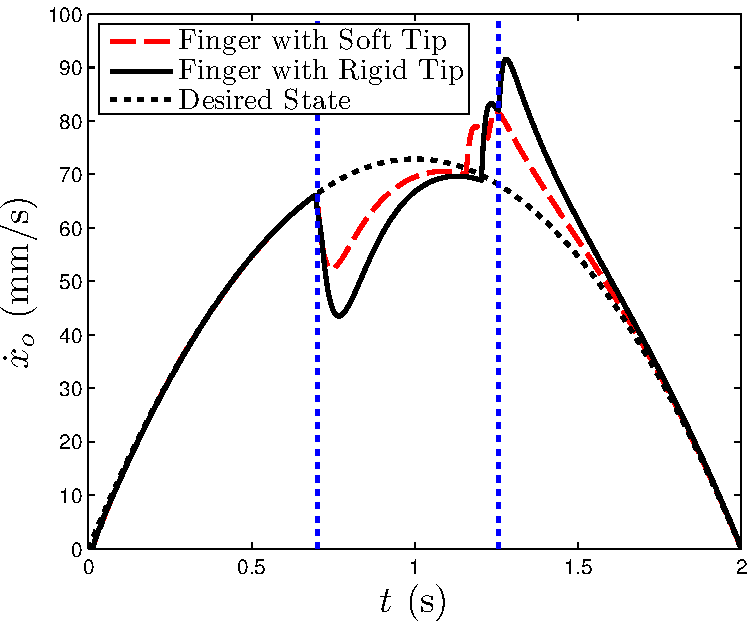
\includegraphics[scale=0.56]{Figures/FigureA.pdf}}
\quad
\subfloat[زیرنویس شکل دوم]{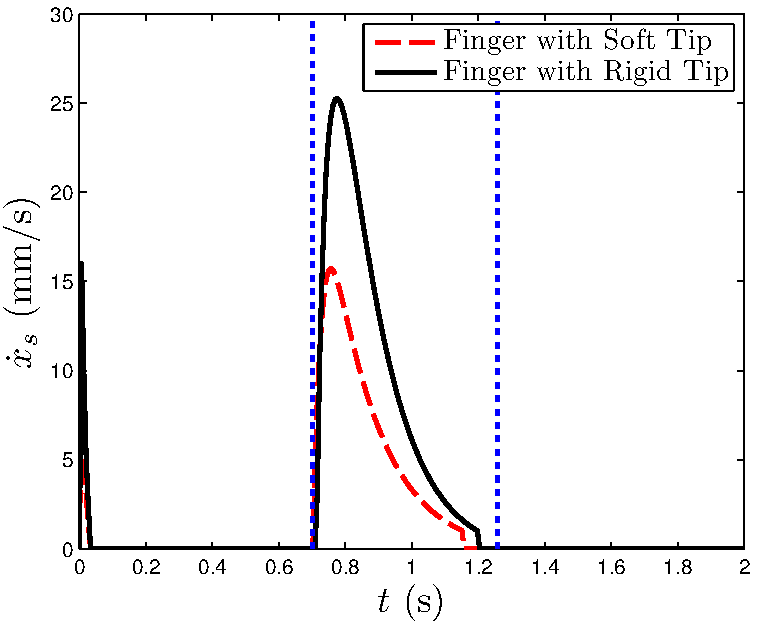
\includegraphics[scale=0.56]{Figures/FigureB.pdf}}
\caption{
قرار دادن دو شکل در کنار یکدیگر، الف) شکل نمونه اول،
ب) شکل نمونه دوم
}
\label{Fig:SampleFigure2_2}
\end{figure}





آیتم‌های مختلف به‌صورت زیر آورده می‌شود:
\begin{itemize}[label=-]
\item
مورد اول
\item
مورد دوم
\item
مورد سوم
\end{itemize}

نمونه‌ای از آیتم‌های شماره‌دار نیز در ادامه آورده شده است. به طور کلی معماری برداشت انرژی به دو دسته‌ی کلی تقسیم می‌شود:
\begin{enumerate}[label=\arabic*)]
\item
برداشت-استفاده:

در این حالت سیستم بلافاصله انرژی برداشت‌شده را مصرف می‌کند. واضح است اگر انرژی کافی در محیط وجود نداشته باشد دستگاه از کار می‌افتد. این نوع سیستم‌ها بیشتر در فشار دادن کلید‌ها، پدال‌ها و دستگاه‌های ردیابی برای انسان‌ها استفاده می‌شود. به طور مثال در پاشنه‌ی کفش دونده‌ای مواد پیزوالکتریک کار گذاشته می‌شود و با فشار پا بر روی کفش و فشرده شدن پیزوالکتریک داخل کفش، انرژی الکتریکی برای ارسال سیگنال 
\lr{RF}
و در نتیجه ردیابی دونده تامین می‌شود. 
\item
برداشت-ذخیره-استفاده:

در این روش سیستم برای ذخیره‌ی انرژی برداشت‌شده به باتری مجهز شده است. این روش برای زمانی‌که انرژی زیادی در محیط وجود داشته باشد و برای منابعی مانند انرژی خورشیدی  کاربرد دارد. روش‌های زیادی برای تبدیل انرژی خورشیدی به انرژی الکتریکی از جمله سلول‌های خورشیدی وجود دارد. در این حالت چگونگی ذخیره‌ی انرژی و بهینه‌سازی مصرف انرژی مطرح می‌شود.
\end{enumerate}




\subsection{زیربخش اول}
نوشته نمونه نوشته نمونه نوشته نمونه نوشته نمونه نوشته نمونه نوشته نمونه نوشته نمونه نوشته نمونه نوشته نمونه نوشته نمونه نوشته نمونه نوشته نمونه نوشته نمونه نوشته نمونه نوشته نمونه نوشته نمونه نوشته نمونه نوشته نمونه نوشته نمونه نوشته نمونه نوشته نمونه نوشته نمونه. در جدول
\ref{Tbl:SampleTable1_2}،
نمونه‌ای از یک جدول واردشده در لاتک و در جدول
\ref{Tbl:SampleTable2_2}،
نمونه‌ای از یک جدول نوشته‌شده در لاتک آورده شده است.

\begin{table}[!htb]
\caption{پارامترهای شبیه‌سازی}
\centering
\begin{tabular}{c}
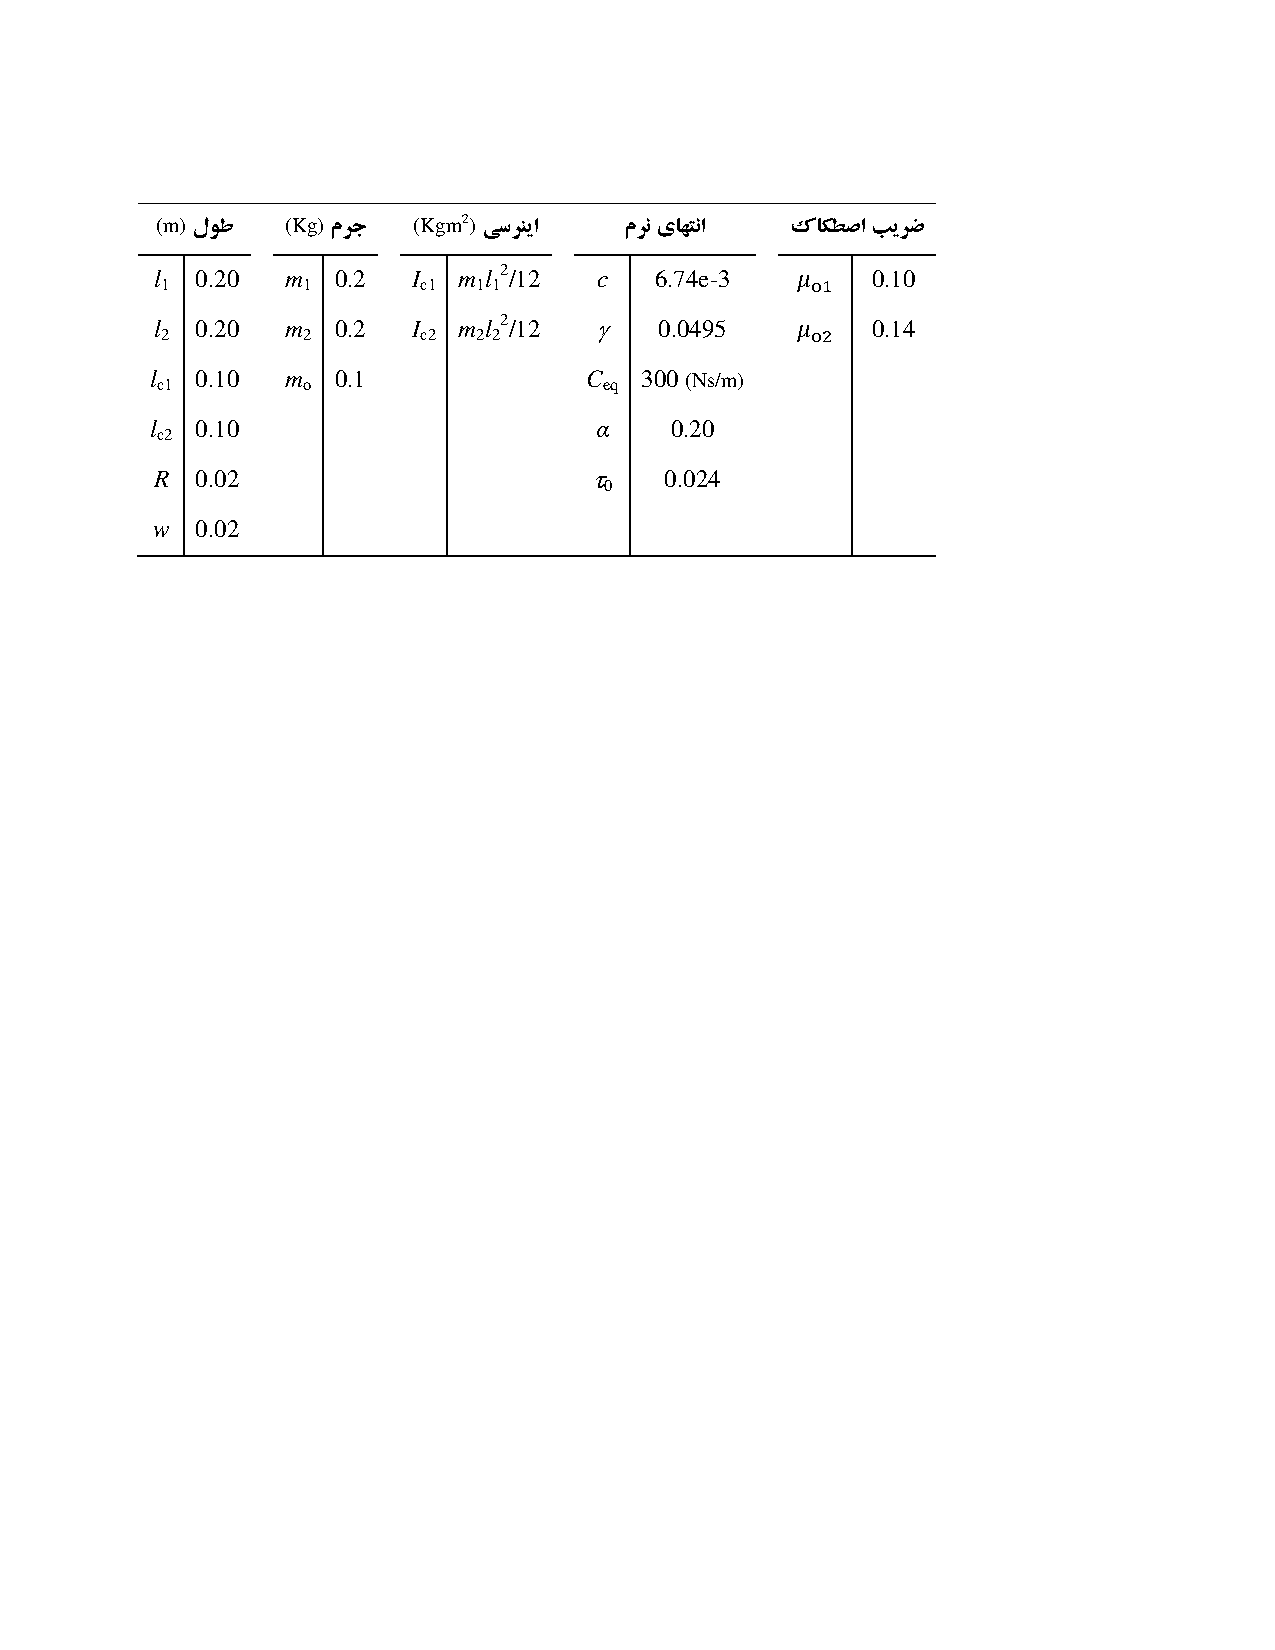
\includegraphics[scale=0.9]{Figures/SampleTable1.pdf} 
\end{tabular}
\vspace{-\baselineskip}
\label{Tbl:SampleTable1_2}
\end{table}

\begin{table}[!htb]
\caption{مقايسه‌ی روش‌هاي برداشت انرژي مبتني بر لرزش‌هاي مکانيکی}
\centering
\begin{tabular}{@{}|p{.15\textwidth}|p{.25\textwidth}|p{.25\textwidth}|p{.25\textwidth}|@{}}
\hline
روش
& 
چگالی انرژی
& 
ابعاد
& 
عیب اصلی
\\ \hline \hline
پیزوالکتریک
& 
$\mathrm{mJ/cm^3}$ 35/4
& 
بزرگ
& 
ولتاژ خروجی کم
\\ \hline
الکترومغناطیس
& 
$\mathrm{mJ/cm^3}$ 24/8
& 
بزرگ
& 
ولتاژ خروجی بسیار کم
\\ \hline
الکترواستاتیک
& 
$\mathrm{mJ/cm^3}$ 4
& 
فشرده در تراشه‌ها
& 
نیاز به منبع شارژ اولیه
\\ \hline
\end{tabular}
\label{Tbl:SampleTable2_2}
\vspace{-\baselineskip}
\end{table}

نمونه‌ای از یک رابطه به‌صورت
\begin{equation}
p\left( r \right) = {C_k}\frac{N}{{\pi {a^2}}}{\left[{1 - {{\left( {\frac{r}{a}} \right)}^k}} \right]^{\frac{1}{k}}},
\label{Eq:Pressure_2}
\end{equation}
است. در رابطه
\ref{Eq:Pressure_2}،
$N$
نیروی عمودی است. نمونه‌ای از استفاده از روابط متوالی به‌صورت
\begin{equation}
\sum \limits_{i = 1}^{k + 1} {E_s}\left( i \right) - T \sum \limits_{i = 1}^k {P_s}\left( i \right) \le B_s^{max},\quad k = 1, \ldots ,N - 1,
\label{Eq:batterysource_2}
\end{equation}\vspace{-\baselineskip}
\begin{equation}
\sum \limits_{i = 1}^{k + 1} {E_r}\left( i \right) - T \sum \limits_{i = 1}^k {P_r}\left( i \right) \le B_r^{max},\quad k = 1, \ldots ,N - 1,
\label{Eq:batteryrellay_2}
\end{equation}
است. نمونه‌ای از یک قضیه و تبصره نیز در ادامه آورده شده است.
\begin{theorem}
اگر ظرفیت باتری‌ها به اندازه کافی بزرگ باشد، جواب بهینه‌ی 
$P_s^*(i)$
و
$P_r^*(i)$
وجود دارد به نحوی که تابع هدف را بیشینه می‌کند و در رابطه‌ی زیر صدق می‌کند:
\begin{equation}
C\left( {{{\left| {{h_{sr}}\left( i \right)} \right|}^2}{P_s}^*\left( i \right)} \right) \ge C\left( {{{\left| {{h_{sd}}\left( i \right)} \right|}^2}{P_s}^*\left( i \right)} \right) + C\left( {{{\left| {{h_{rd}}\left( {i + 1} \right)} \right|}^2}P_r^*\left( {i} \right)} \right).
\label{Eq:theorem1_2}
\end{equation}

\begin{proof}
بار دیگر فرم تابع هدف را در نظر می‌گیریم. لازم به ذکر است اینجا تابع هدف یک تابع دومتغیره است.
\begin{equation}
{R({\mathbf{P}_s},{\mathbf{P}_r}) = {\frac{1}{2}\sum\limits_{i = 1}^N {\min } \left\{ {C\left( {{{\left| {{h_{sr}}\left( i \right)} \right|}^2}{P_s}\left( i \right)} \right),} C\left( {{{\left| {{h_{sd}}\left( i \right)} \right|}^2}{P_s}\left( i \right)} \right) \right\} }}.
\end{equation}
حال بلوک
$i$ام
را در نظر می‌گیریم. اگر رابطه‌ی
\ref{Eq:theorem1_2}
برای
$i$
برقرار نباشد، به عبارت دیگر اگر داشته باشیم،
\begin{equation}
C\left( {{{\left| {{h_{sr}}\left( i \right)} \right|}^2}{P_s}^*\left( i \right)} \right) < C\left( {{{\left| {{h_{sd}}\left( i \right)} \right|}^2}{P_s}^*\left( i \right)} \right) + C\left( {{{\left| {{h_{rd}}\left( {i + 1} \right)} \right|}^2}P_r^*\left( {i + 1} \right)} \right),
\label{Eq:theorem1(2)_2}
\end{equation}
بنابراین
\begin{equation}
C\left( {{{\left| {{h_{sr}}\left( i \right)} \right|}^2}{P_s}^*\left( i \right)} \right)+ C\left( {{{\left| {{h_{sd}}\left( i \right)} \right|}^2}{P_s}^*\left( i \right)} \right) =C\left( {{{\left| {{h_{sr}}\left( i \right)} \right|}^2}{P_s}^*\left( i \right)} \right).
\end{equation}
پس در تابع هدف مسئله، مقدار بهینه‌ی مسئله برابر عبارت سمت چپ رابطه‌ی
\ref{Eq:theorem1(2)_2}
شده است و آرگومان دوم و  هم‌چنین مقدار
$P_r^*(i)$
هیچ نقشی در مقدار بهینه ندارد. بنابراین می‌توانیم 
$P_r^*(i)$
را آنقدر کاهش دهیم تا در رابطه‌ی
\ref{Eq:theorem1(2)_2}
تساوی برقرار شود بدون آنکه مقدار بهینه‌ی مسئله تغییر کند.
\end{proof}
\label{theorem1_2}
\end{theorem}

\begin{remark}
از قضیه‌ی
\ref{theorem1_2}
نتیجه می‌گیریم که جواب بهینه‌ی مسئله‌ی
\lr{P}
در حالت کلی یکتا نیست. به طور مثال وقتی مقدار انرژی برداشت‌شده در رله خیلی بیشتر از این انرژی در منبع باشد مسئله می‌تواند جواب‌های زیادی داشته باشد. بنابراین همواره می‌توان برای صرفه‌جویی در مصرف انرژی، بدون کاهش مقدار نرخ گذردهی سیستم، کمترین مقدار توان را برای رله انتخاب کرد. بنابراین با توجه به رابطه
\begin{equation}
C\left( {{{\left| {{h_{sr}}\left( i \right)} \right|}^2}{P_s}^*\left( i \right)} \right) 
\ge C\left( {{{\left| {{h_{sd}}\left( i \right)} \right|}^2}{P_s}^*\left( i \right)} \right) + C\left( {{{\left| {{h_{rd}}\left( {i} \right)} \right|}^2}P_r^*\left( {i} \right)} \right),
\label{Eq:remark1_2}
\end{equation}
و با  استفاده از رابطه
\ref{Eq:remark1_2}
خواهیم داشت،
\begin{equation}
{R_r}(i) = \min \left\{ {C\left( {{{\left| {{h_{rd}}(i)} \right|}^2}{P_r}(i)} \right),C\left( {{{\left| {{h_{sr}}(i)} \right|}^2}{P_s}(i)} \right)} \right\}.
\end{equation}

بنابراین می‌توان با انتخاب کمترین توان و نرخ برای رله از مصرف بی‌رویه‌ی انرژی جلوگیری کرد. فرض بزرگ بودن ظرفیت باتری‌ به این دلیل است که اگر ظرفیت باتری محدود باشد برای کاهش
$P_r^*(i)$
با محدودیت مواجه هستیم. چون در صورت کاهش بی از حد توان رله ممکن است از ناحیه‌ی شدنی مسئله خارج شویم. به هر حال برای هر دو حالت ظرفیت نامحدود و محدود باتری جواب مسئله یکتا نیست و همواره می‌توان با کاهش توان رله مصرف انرژی را کاهش داد.
\end{remark}





\chapter{نتیجه‌گیری و پیشنهادها}
\section{‌نتیجه‌گیری}
نوشته نمونه نوشته نمونه نوشته نمونه نوشته نمونه نوشته نمونه نوشته نمونه نوشته نمونه نوشته نمونه نوشته نمونه نوشته نمونه نوشته نمونه نوشته نمونه نوشته نمونه نوشته نمونه نوشته نمونه نوشته نمونه نوشته نمونه نوشته نمونه نوشته نمونه نوشته نمونه نوشته نمونه نوشته نمونه. نوشته نمونه نوشته نمونه نوشته نمونه نوشته نمونه نوشته نمونه نوشته نمونه نوشته نمونه نوشته نمونه نوشته نمونه نوشته نمونه نوشته نمونه نوشته نمونه نوشته نمونه نوشته نمونه نوشته نمونه نوشته نمونه نوشته نمونه نوشته نمونه نوشته نمونه نوشته نمونه نوشته نمونه نوشته نمونه. نوشته نمونه نوشته نمونه نوشته نمونه نوشته نمونه نوشته نمونه نوشته نمونه نوشته نمونه نوشته نمونه نوشته نمونه نوشته نمونه نوشته نمونه نوشته نمونه نوشته نمونه نوشته نمونه نوشته نمونه نوشته نمونه نوشته نمونه نوشته نمونه نوشته نمونه نوشته نمونه نوشته نمونه نوشته نمونه. نوشته نمونه نوشته نمونه نوشته نمونه نوشته نمونه نوشته نمونه نوشته نمونه نوشته نمونه نوشته نمونه نوشته نمونه نوشته نمونه نوشته نمونه نوشته نمونه نوشته نمونه نوشته نمونه نوشته نمونه نوشته نمونه نوشته نمونه نوشته نمونه نوشته نمونه نوشته نمونه نوشته نمونه نوشته نمونه. نوشته نمونه نوشته نمونه نوشته نمونه نوشته نمونه نوشته نمونه نوشته نمونه نوشته نمونه نوشته نمونه نوشته نمونه نوشته نمونه نوشته نمونه نوشته نمونه نوشته نمونه نوشته نمونه نوشته نمونه نوشته نمونه نوشته نمونه نوشته نمونه نوشته نمونه نوشته نمونه نوشته نمونه نوشته نمونه. نوشته نمونه نوشته نمونه نوشته نمونه نوشته نمونه نوشته نمونه نوشته نمونه نوشته نمونه نوشته نمونه نوشته نمونه نوشته نمونه نوشته نمونه نوشته نمونه نوشته نمونه نوشته نمونه نوشته نمونه نوشته نمونه نوشته نمونه نوشته نمونه نوشته نمونه نوشته نمونه نوشته نمونه نوشته نمونه. نوشته نمونه نوشته نمونه نوشته نمونه نوشته نمونه نوشته نمونه نوشته نمونه نوشته نمونه نوشته نمونه نوشته نمونه نوشته نمونه نوشته نمونه نوشته نمونه نوشته نمونه نوشته نمونه نوشته نمونه نوشته نمونه نوشته نمونه نوشته نمونه نوشته نمونه نوشته نمونه نوشته نمونه نوشته نمونه.

\section{پیشنهادها}
نوشته نمونه نوشته نمونه نوشته نمونه نوشته نمونه نوشته نمونه نوشته نمونه نوشته نمونه نوشته نمونه نوشته نمونه نوشته نمونه نوشته نمونه نوشته نمونه نوشته نمونه نوشته نمونه نوشته نمونه نوشته نمونه نوشته نمونه نوشته نمونه نوشته نمونه نوشته نمونه نوشته نمونه نوشته نمونه. نوشته نمونه نوشته نمونه نوشته نمونه نوشته نمونه نوشته نمونه نوشته نمونه نوشته نمونه نوشته نمونه نوشته نمونه نوشته نمونه نوشته نمونه نوشته نمونه نوشته نمونه نوشته نمونه نوشته نمونه نوشته نمونه نوشته نمونه نوشته نمونه نوشته نمونه نوشته نمونه نوشته نمونه نوشته نمونه. نوشته نمونه نوشته نمونه نوشته نمونه نوشته نمونه نوشته نمونه نوشته نمونه نوشته نمونه نوشته نمونه نوشته نمونه نوشته نمونه نوشته نمونه نوشته نمونه نوشته نمونه نوشته نمونه نوشته نمونه نوشته نمونه نوشته نمونه نوشته نمونه نوشته نمونه نوشته نمونه نوشته نمونه نوشته نمونه. نوشته نمونه نوشته نمونه نوشته نمونه نوشته نمونه نوشته نمونه نوشته نمونه نوشته نمونه نوشته نمونه نوشته نمونه نوشته نمونه نوشته نمونه نوشته نمونه نوشته نمونه نوشته نمونه نوشته نمونه نوشته نمونه نوشته نمونه نوشته نمونه نوشته نمونه نوشته نمونه نوشته نمونه نوشته نمونه. نوشته نمونه نوشته نمونه نوشته نمونه نوشته نمونه نوشته نمونه نوشته نمونه نوشته نمونه نوشته نمونه نوشته نمونه نوشته نمونه نوشته نمونه نوشته نمونه نوشته نمونه نوشته نمونه نوشته نمونه نوشته نمونه نوشته نمونه نوشته نمونه نوشته نمونه نوشته نمونه نوشته نمونه نوشته نمونه. نوشته نمونه نوشته نمونه نوشته نمونه نوشته نمونه نوشته نمونه نوشته نمونه نوشته نمونه نوشته نمونه نوشته نمونه نوشته نمونه نوشته نمونه نوشته نمونه نوشته نمونه نوشته نمونه نوشته نمونه نوشته نمونه نوشته نمونه نوشته نمونه نوشته نمونه نوشته نمونه نوشته نمونه نوشته نمونه. نوشته نمونه نوشته نمونه نوشته نمونه نوشته نمونه نوشته نمونه نوشته نمونه نوشته نمونه نوشته نمونه نوشته نمونه نوشته نمونه نوشته نمونه نوشته نمونه نوشته نمونه نوشته نمونه نوشته نمونه نوشته نمونه نوشته نمونه نوشته نمونه نوشته نمونه نوشته نمونه نوشته نمونه نوشته نمونه.

% ░░░░░░░▒▒▒▒▒▒▓▓▓▓ Appendices ▓▓▓▓▒▒▒▒▒▒░░░░░░░
\MakeAppendices
\section{جزئیات معادله‌ها}
نوشته نمونه نوشته نمونه نوشته نمونه نوشته نمونه نوشته نمونه نوشته نمونه نوشته نمونه نوشته نمونه نوشته نمونه نوشته نمونه نوشته نمونه نوشته نمونه نوشته نمونه نوشته نمونه نوشته نمونه نوشته نمونه نوشته نمونه نوشته نمونه نوشته نمونه نوشته نمونه نوشته نمونه نوشته نمونه. نوشته نمونه نوشته نمونه نوشته نمونه نوشته نمونه نوشته نمونه نوشته نمونه نوشته نمونه نوشته نمونه نوشته نمونه نوشته نمونه نوشته نمونه نوشته نمونه نوشته نمونه نوشته نمونه نوشته نمونه نوشته نمونه نوشته نمونه نوشته نمونه نوشته نمونه نوشته نمونه نوشته نمونه نوشته نمونه. نوشته نمونه نوشته نمونه نوشته نمونه نوشته نمونه نوشته نمونه نوشته نمونه نوشته نمونه نوشته نمونه نوشته نمونه نوشته نمونه نوشته نمونه نوشته نمونه نوشته نمونه نوشته نمونه نوشته نمونه نوشته نمونه نوشته نمونه نوشته نمونه نوشته نمونه نوشته نمونه نوشته نمونه نوشته نمونه. نوشته نمونه نوشته نمونه نوشته نمونه نوشته نمونه نوشته نمونه نوشته نمونه نوشته نمونه نوشته نمونه نوشته نمونه نوشته نمونه نوشته نمونه نوشته نمونه نوشته نمونه نوشته نمونه نوشته نمونه نوشته نمونه نوشته نمونه نوشته نمونه نوشته نمونه نوشته نمونه نوشته نمونه نوشته نمونه. نوشته نمونه نوشته نمونه نوشته نمونه نوشته نمونه نوشته نمونه نوشته نمونه نوشته نمونه نوشته نمونه نوشته نمونه نوشته نمونه نوشته نمونه نوشته نمونه نوشته نمونه نوشته نمونه نوشته نمونه نوشته نمونه نوشته نمونه نوشته نمونه نوشته نمونه نوشته نمونه نوشته نمونه نوشته نمونه. نوشته نمونه نوشته نمونه نوشته نمونه نوشته نمونه نوشته نمونه نوشته نمونه نوشته نمونه نوشته نمونه نوشته نمونه نوشته نمونه نوشته نمونه نوشته نمونه نوشته نمونه نوشته نمونه نوشته نمونه نوشته نمونه نوشته نمونه نوشته نمونه نوشته نمونه نوشته نمونه نوشته نمونه نوشته نمونه. نوشته نمونه نوشته نمونه نوشته نمونه نوشته نمونه نوشته نمونه نوشته نمونه نوشته نمونه نوشته نمونه. نمونه‌ای از یک رابطه به‌صورت
\begin{equation}
p\left( r \right) = {C_k}\frac{N}{{\pi {a^2}}}{\left[{1 - {{\left( {\frac{r}{a}} \right)}^k}} \right]^{\frac{1}{k}}}
\label{Eq:Pressure1}
\end{equation}
است.

\newpage
\section{اثبات روابط ریاضی}
نوشته نمونه نوشته نمونه نوشته نمونه نوشته نمونه نوشته نمونه نوشته نمونه نوشته نمونه نوشته نمونه نوشته نمونه نوشته نمونه نوشته نمونه نوشته نمونه نوشته نمونه نوشته نمونه نوشته نمونه نوشته نمونه نوشته نمونه نوشته نمونه نوشته نمونه نوشته نمونه نوشته نمونه نوشته نمونه. نوشته نمونه نوشته نمونه نوشته نمونه نوشته نمونه نوشته نمونه نوشته نمونه نوشته نمونه نوشته نمونه نوشته نمونه نوشته نمونه نوشته نمونه نوشته نمونه نوشته نمونه نوشته نمونه نوشته نمونه نوشته نمونه نوشته نمونه نوشته نمونه نوشته نمونه نوشته نمونه نوشته نمونه نوشته نمونه. نوشته نمونه نوشته نمونه نوشته نمونه نوشته نمونه نوشته نمونه نوشته نمونه نوشته نمونه نوشته نمونه نوشته نمونه نوشته نمونه نوشته نمونه نوشته نمونه نوشته نمونه نوشته نمونه نوشته نمونه نوشته نمونه نوشته نمونه نوشته نمونه نوشته نمونه نوشته نمونه نوشته نمونه نوشته نمونه. (شکل~%
\ref{Fig:World1})
نوشته نمونه نوشته نمونه نوشته نمونه نوشته نمونه نوشته نمونه نوشته نمونه نوشته نمونه نوشته نمونه نوشته نمونه نوشته نمونه نوشته نمونه نوشته نمونه نوشته نمونه نوشته نمونه نوشته نمونه نوشته نمونه نوشته نمونه نوشته نمونه نوشته نمونه نوشته نمونه نوشته نمونه نوشته نمونه. نوشته نمونه نوشته نمونه نوشته نمونه نوشته نمونه نوشته نمونه نوشته نمونه نوشته نمونه نوشته نمونه نوشته نمونه نوشته نمونه نوشته نمونه نوشته نمونه نوشته نمونه نوشته نمونه نوشته نمونه نوشته نمونه نوشته نمونه نوشته نمونه نوشته نمونه نوشته نمونه نوشته نمونه نوشته نمونه. نوشته نمونه نوشته نمونه نوشته نمونه نوشته نمونه نوشته نمونه نوشته نمونه نوشته نمونه نوشته نمونه نوشته نمونه نوشته نمونه نوشته نمونه نوشته نمونه نوشته نمونه نوشته نمونه نوشته نمونه نوشته نمونه نوشته نمونه نوشته نمونه نوشته نمونه نوشته نمونه نوشته نمونه نوشته نمونه.
\begin{figure}[!htb]
\centering
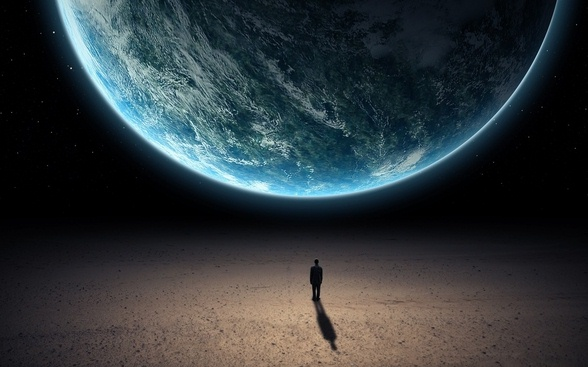
\includegraphics[scale=0.4]{Figures/World.jpg}
\caption{تصویر مفهومی}
\label{Fig:World1}
\end{figure}

نوشته نمونه نوشته نمونه نوشته نمونه نوشته نمونه نوشته نمونه نوشته نمونه نوشته نمونه نوشته نمونه نوشته نمونه نوشته نمونه نوشته نمونه نوشته نمونه نوشته نمونه نوشته نمونه نوشته نمونه نوشته نمونه نوشته نمونه نوشته نمونه نوشته نمونه نوشته نمونه نوشته نمونه نوشته نمونه.

% ░░░░░░░▒▒▒▒▒▒▓▓▓▓ References ▓▓▓▓▒▒▒▒▒▒░░░░░░░
\MakeReferences
\bibliographystyle{Settings/ModifiedIEEEtranFa}
\bibliography{References}

% ░░░░░░░▒▒▒▒▒▒▓▓▓▓ Abstract - English ▓▓▓▓▒▒▒▒▒▒░░░░░░░
\DepartmentEn{Department of Mechanical Engineering}
\DegreeEn{Doctor of Philosophy (PhD)} % Or \DegreeEn{Master of Science (MSc)} 
\YourFullnameEn{Amin Fakhari}
\YourEmailAddress{a.fakhari@me.iut.ac.ir}
\DateEn{December 27, 2015}
\FirstSupervisorEn{Mehdi Keshmiri, Prof.}
\FirstSupervisorEmailAddress{user1@cc.iut.ac.ir}
\SecondSupervisorEn{Second Supervisor, Prof.} % Optional (Remove It If You Don't Have)
\SecondSupervisorEmailAddress{user2@cc.iut.ac.ir} % Optional (Remove It If You Don't Have)
\TitleEn{Slippage Analysis and Control in Manipulation of Objects \\[0.2cm] in Contact with Even Surfaces Using Soft Fingers}
% اگر عنوان رساله طولانی بود، در دو خط به صورت نشان داده شده تقسیم شود.

\AbstractEn{
At this section, English abstract is written. At this section, English abstract is written. At this section, English abstract is written. At this section, English abstract is written. At this section, English abstract is written. At this section, English abstract is written. At this section, English abstract is written. At this section, English abstract is written. At this section, English abstract is written. At this section, English abstract is written. At this section, English abstract is written. At this section, English abstract is written. At this section, English abstract is written. At this section, English abstract is written. At this section, English abstract is written. At this section, English abstract is written. At this section, English abstract is written. At this section, English abstract is written. At this section, English abstract is written. At this section, English abstract is written. At this section, English abstract is written. At this section, English abstract is written. At this section, English abstract is written. At this section, English abstract is written. At this section, English abstract is written. At this section, English abstract is written. At this section, English abstract is written. At this section, English abstract is written. At this section, English abstract is written. At this section, English abstract is written. At this section, English abstract is written. At this section, English abstract is written. At this section, English abstract is written. At this section, English abstract is written. At this section, English abstract is written. At this section, English abstract is written. At this section, English abstract is written. At this section, English abstract is written. At this section, English abstract is written. At this section, English abstract is written. At this section, English abstract is written. At this section, English abstract is written. At this section, English abstract is written. At this section, English abstract is written.
}

\KeywordsEn{1- First Keyword, 2- Second Keyword, 3- Third Keyword, 4- Fourth Keyword, 5- Fifth Keyword}

\MakeEnglishAbstract

% ░░░░░░░▒▒▒▒▒▒▓▓▓▓ Signature - English ▓▓▓▓▒▒▒▒▒▒░░░░░░░
\FirstAdvisorEn{First Advisor, Assoc. Prof.}
\SecondAdvisorEn{Second Advisor, Assist. Prof.} % Optional (Remove It If You Don't Have)
\FirstExaminerEn{First Examiner, Prof.}
\SecondExaminerEn{Second Examiner, Prof.} % Optional (Remove It If You Don't Have)
\ThirdExaminerEn{Third Examiner, Prof.} % Optional (Remove It If You Don't Have)
\FourthExaminerEn{Fourth Examiner, Prof.} % Optional (Remove It If You Don't Have)
\FifthExaminerEn{Fifth Examiner, Prof.} % Optional (Remove It If You Don't Have)
\DeanOfDepartmentEn{Dean, Prof.}

\MakeEnglishSignaturePage

\end{document} 
